\section{Introduction}
\label{sec:intro}


\begin{figure}[b!]
    \vspace{-8mm}
    \centering
    \begin{subfigure}[c]{0.41\linewidth}
        \centering
        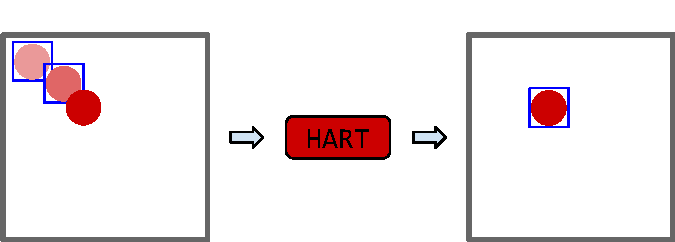
\includegraphics[width=\linewidth]{figures/MOHART/system_hart}
        \vspace{-5mm}
        \caption{HART}
    \end{subfigure}
    \hspace{20mm}
    \begin{subfigure}[c]{0.41\linewidth}
        \centering
        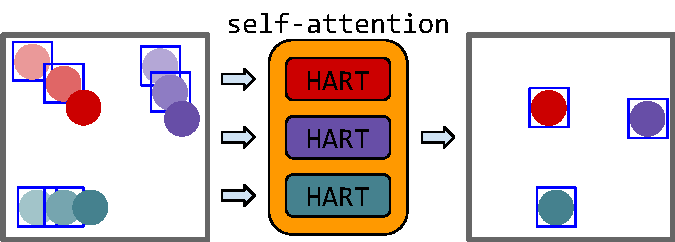
\includegraphics[width=\linewidth]{figures/MOHART/system_mohart}
        \vspace{-5mm}
        \caption{MOHART}
    \end{subfigure}
    \vspace{-2mm}
    \caption{
    Single-object tracking with \gls{HART} (left) and our extension to multi-object tracking (\gls{MOHART}, right). In our proposed framework, the different \gls{HART} trackers are connected via a relational reasoning module allowing for more robust tracking and more accurate future trajectory prediction.
    % \vspace{-4mm}
    }
    \label{fig:teaser}
\end{figure}

Autonomous vehicles need to operate in rich environments that contain a large variety of interacting object. 
%
This variety motivates the need for \emph{class-agnostic} object trackers, which break with the popular tracking-by-detection paradigm \cite{Zhang2008,Milan2014,bae2017confidence, keuper2018motion}. 
%
In tracking-by-detection, static video frames are first analysed by an object detector,\eg a pre-trained deep \gls{CNN} such as \textsc{yolo} \citep{Redmon15}, and then the detected objects are linked across frames. 
%
Algorithms from this family can achieve high accuracy, provided sufficient labelled data to train the object detector, and given that all encountered objects can be associated with known classes. 
%

\Gls{HART} is a recently proposed alternative for single-object tracking (\textsc{sot}), where an arbitrary object can be tracked from an initial video frame \citep{Kosiorek17}.
%
Since the initial bounding-box is user-provided and may be placed over any part of the image, regardless of whether it corresponds to an object and its class, \gls{HART} can track arbitrary objects.
% 
\Gls{HART} efficiently processes just the relevant part of an image using spatial attention; it also integrates object detection, feature extraction, and motion modelling into one network, which is trained fully end-to-end.
Contrary to tracking-by-detection, where only one video frame is typically processed at any given time to generate bounding box proposals, end-to-end learning in \gls{HART} allows discovering complex visual and spatio-temporal patterns in videos, which is conducive to inferring what an object is and how it moves.
%

In the original formulation, \gls{HART} is limited to the single-object modality---as are other existing end-to-end trackers \cite{Kahou15,Danesh19,Gordon2018}.
%
In this work, we present \gls{MOHART}, a class-agnostic tracker with complex relational reasoning capabilities provided by a multi-headed self-attention module \citep{Vaswani17,Lee2019settransformer}. 
\Gls{MOHART} infers the latent state of every tracked object in parallel, and uses self-attention to inform per-object states about other tracked objects.
This helps to avoid performance loss under self-occlusions of tracked objects or strong ego-motion.
Moreover, since the model is trained end-to-end, it is able to learn how to manage faulty or missing sensor inputs.
It can also use the inferred objects' states to predict their future trajectories, which depend on interactions between different objects. See \cref{fig:teaser} for a high-level illustration of \gls{HART} and \gls{MOHART}.

After describing related work in \Cref{sec:related} and the methodology in \cref{sec:method}, we employ the algorithm on toy domains to validate its efficacy in \Cref{sec:experiment_toy}. By controlling the stochasticity of toy environments, we show that single-object tracking is sufficient in some cases, even those featuring strong long-range interactions, while it may fail in other cases.
This may hint at a similar phenomenon in the real world: tracking objects or predicting their future motion independently may be possible in most (but not all) cases, while solving the remaining corner cases might require taking interactions between objects into account.
It is these corner cases that motivate our work.
In \Cref{sec:experiment_real}, we test \gls{MOHART} on three real world datasets (MOTChallenge \cite{MOT16}, UA-DETRAC \cite{Wen15}, Stanford Drone dataset \cite{DroneDataset}) and show that relational reasoning between objects is most important on the MOTChallenge dataset. We hypothesise that this is due to its richness in ego-motion, occlusions and crowded scenes---a result supported by our ablation study. Furthermore, we show that \gls{MOHART} is able to gracefully handle missing sensory inputs---without any architectural changes. In this case, it falls back on its internal motion model, which also allows for accurate prediction of object locations multiple time steps into the future, learned in a data-driven manner.


